% !TEX TS-program = pdflatexmk
\documentclass{article}
\usepackage[latin1]{inputenc} 

\newenvironment{Ncenter}{%
  \setlength\topsep{-10pt}
  \setlength\parskip{-100pt}
  \begin{center}
}{%
  \end{center}
}


\newcommand{\kmo}{k_{\mathrm{OT \to O+T}}}
\newcommand{\kOpT}{k_{\mathrm{O+T \to OT}}}
\newcommand{\kmt}{k_{\mathrm{OTE \to OT+E}}}
\newcommand{\kt}{k_{\mathrm{OT+E \to OTE}}}
\newcommand{\kE}{k_{\mathrm{OTE \to OCE}}}
\newcommand{\kD}{k_{\mathrm{OC \to O+C}}}
\newcommand{\vp}{v_{\mathrm{prod}}}
\newcommand{\vd}{k_{\mathrm{T \to \emptyset}}}
\newcommand{\Trel}{T_{\rm{rel}}}
\newcommand{\EC}{EC_{\rm{50}}}
\newcommand{\KdOT}{K_{\mathrm{dOT}}}
\newcommand{\Trelmin}{T_{\rm{rel,min}}}

\usepackage[labelsep=none]{caption}
\renewcommand{\thefigure}{}

\title{R-code for producing Figure 2 from Pedersen et al. (2013)}
\author{Lykke Pedersen, \and Peter H Hagedorn, \and Marie Lindholm, \and Morten Lindow}
\date{}

\usepackage{Sweave}
\begin{document}
\Sconcordance{concordance:Vignette2.tex:Vignette2.Rnw:%
1 33 1 1 0 6 1 1 2 1 0 1 2 4 0 1 2 3 1 1 3 2 0 1 2 1 0 1 1 3 0 2 2 4 0 %
2 2 1 0 1 2 1 0 1 2 1 1 1 3 1 0 1 6 5 0 1 1 1 2 1 0 3 1 1 3 2 0 1 3 2 0 %
1 3 2 0 1 3 2 0 1 3 5 0 1 2 8 1 1 2 1 0 1 3 2 0 2 1 1 2 1 0 2 1 3 0 1 2 %
9 1 1 2 1 0 1 1 3 0 2 2 1 0 2 1 3 0 2 2 1 0 1 2 1 0 2 1 1 2 1 0 1 1 3 0 %
1 2 8 1 1 2 1 0 3 1 1 3 1 0 1 1 2 2 1 3 2 0 1 2 6 1 1 2 1 0 2 1 3 0 1 2 %
7 1 1 3 2 0 1 1 1 2 1 1 1 2 1 0 1 2 1 0 1 2 1 3 2 0 5 1 1 2 1 0 2 1 3 0 %
1 2 7 1 1 3 2 0 1 1 3 2 1 0 1 1 1 2 7 1 1 2 1 0 2 1 3 0 1 2 77 1}



\maketitle
This vignette includes the commands to reproduce Fig. 2 from ``A kinetic model explains why shorter and less
affine enzyme-recruiting oligonucleotides can be
more potent". The R-functions from the ASOmodels package are used.
\begin{Schunk}
\begin{Sinput}
> require(devtools)
> #install_github('ASOmodel',username='lykkep')
> require(ASOmodels)
\end{Sinput}
\end{Schunk}

%%%%%%%%%%%%%%%%%%%%%%%%%%%%%%%%%%%%%%%%%%%%%%%%%%%%%%%%%%%%%%%%%%%%%%%%%%
\section*{Kinetic model figures}

%%%%%%%%%%%%%%%%%%%%%%%%%%%%%%%%%%%%%%%%%%%%%%%%%%%%%%%%%%%%%%%%%%%%%%%%%%
\subsection*{Figure 2a: Time-resolved simulation of the model (unsaturated)}
Parameters for the model, the initial concentrations and the time-steps for which the simulation is performed:
\begin{Schunk}
\begin{Sinput}
> parms <- c(Et = 1,KdOT = 0.3,kOpT = 0.2,KdOTE = 70,kOTpE = 5,  
+            vprod = 0.2,kdegrad = 0.04,alpha=0.1,kcleav = 8)
> init <- c(T=parms['vprod']/parms['kdegrad'], OT=0, OTE=0, 
+           E=parms['Et'], O=0.1, OCE=0, OC=0)
\end{Sinput}
\end{Schunk}
Using \texttt{vode()} the model is simulated in time. The function \texttt{diffASO()} is part of the ASOmodels package. 
\begin{Schunk}
\begin{Sinput}
> solASO <- vode(init,0:100,diffASO,parms)
\end{Sinput}
\end{Schunk}
The timetraces for the concentrations of $[O]$, $[T]$, $[OT]$, $[OTE]$, and $[E]$ are plotted:
\begin{Schunk}
\begin{Sinput}
> colVAR <- c("black","darkgreen","darkred","orange","green")  
> SSvalue <- signif(last(solASO),3) 
> SSvalue[c(3:4,6)] <- SSvalue[c(3:4,6)]*1E3
> xtime <- 59; ySS <- c(0.08,0.88,0.83,0.18,0.13)
> uSS <- c('nM','pM','pM','nM','pM')
> labSS=c('T','OT','OTE','E','O')
> par(mar=c(3.2,3.4,0.1,0.1),bty='n',mgp=c(2,0.7,0),
+     las=1,cex.lab=1.25)
> plot(0,0,ylim=c(0,1),xlim=c(0,xtime+30),type='n',xaxt='n',
+      yaxt='n',ylab='relative concentrations',xlab='minutes')
> axis(2,at=c(0,1),label=c('min','max'),las=1)
> axis(1,at=c(seq(0,xtime,by=10),xtime+20),
+      label=c(seq(0,xtime,by=10),''))
> axis(1,at=xtime+20,label='steady-\nstate',mgp=c(0,1.6,0))
> for(i in 2:6){ 
+   par(new=TRUE)
+   plot(solASO[1:(xtime+1),1], solASO[1:(xtime+1),i], xaxt='n',
+        yaxt='n',ylim=range(solASO[,i]),col=colVAR[i-1], 
+        type='l',ylab=NA,xlab=NA,xlim=c(0,xtime+30)) 
+   lines(xtime+5:37,rep(solASO[101,i],33),col=colVAR[(i-1)]) 
+   y <- diff(par('usr')[3:4])*ySS[i-1]+par('usr')[3]
+   text(xtime+5,y,col=colVAR[i-1],adj=0,cex=0.8,
+        substitute(b==e*l,list(e=SSvalue[i],l=uSS[i-1],b=labSS[i-1]) ))
+ }
\end{Sinput}
\end{Schunk}
\begin{figure}[!h]
\begin{Ncenter}
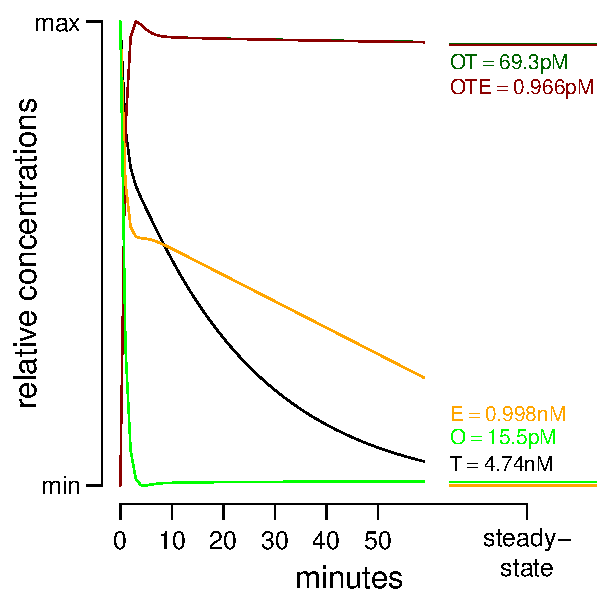
\includegraphics[width=0.5\textwidth]{Vignette2-Figa}
\end{Ncenter}
\caption{2a: Time resolved simulation of the relative concentrations of key species.}
\end{figure}

%%%%%%%%%%%%%%%%%%%%%%%%%%%%%%%%%%%%%%%%%%%%%%%%%%%%%%%%%%%%%%%%%%%%%%%%%%
\subsection*{Figure 2b: Time-resolved simulation of the model (saturated)}
The initial oligonucleotide concentration is increased to 100nM.
\begin{Schunk}
\begin{Sinput}
> init <- c(T=parms['vprod']/parms['kdegrad'], OT=0, OTE=0, 
+           E=parms['Et'], O=100, OCE=0, OC=0)
> solASO <- vode(init,0:100,diffASO,parms)
\end{Sinput}
\end{Schunk}
The timetraces for the concentrations of $[O]$, $[T]$, $[OT]$, $[OTE]$, and $[E]$ are plotted:
\begin{Schunk}
\begin{Sinput}
> SSvalue <- signif(last(solASO),3)
> SSvalue[c(2,4)] <- SSvalue[c(2,4)]*1E3
> xtime <- 55; ySS <- c(0.06,0.3,0.34,0.26,0.67)
> uSS <- c('pM','nM','pM',rep('nM',2)) 
> labSS=c('T','OT','OTE','E','O')
> par(mar=c(3.2,3.4,0.1,0.1),bty='n',mgp=c(2,0.7,0),
+     las=1,cex.lab=1.25)
> plot(0,0,ylim=c(0,1),xlim=c(0,xtime+25),type='n',xaxt='n',
+      yaxt='n',ylab='relative concentrations',xlab='minutes')
> axis(2,at=c(0,1),label=c('min','max'),las=1)
> axis(1,at=c(seq(0,xtime,by=10),xtime+15),
+      label=c(seq(0,xtime,by=10),''))
> axis(1,at=xtime+15,label='steady-\nstate',mgp=c(0,1.6,0))
> for(i in 2:6){ 
+   par(new=TRUE)
+   plot(solASO[1:(xtime+1),1], solASO[1:(xtime+1),i], xaxt='n',
+        yaxt='n',ylim=range(solASO[,i]),col=colVAR[i-1], 
+        type='l',ylab=NA,xlab=NA,xlim=c(0,xtime+25)) 
+   lines(xtime+5:25,rep(solASO[101,i],21),col=colVAR[(i-1)]) 
+   y <- diff(par('usr')[3:4])*ySS[i-1]+par('usr')[3]
+   text(xtime+5,y,col=colVAR[i-1],adj=0,cex=0.8,
+        substitute(b==e*l,list(e=SSvalue[i],l=uSS[i-1],b=labSS[i-1])))
+ }
\end{Sinput}
\end{Schunk}
\begin{figure}[!h]
\begin{Ncenter}
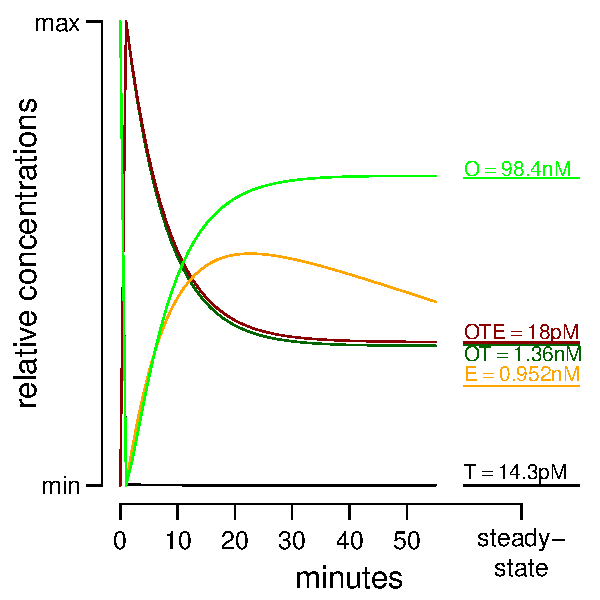
\includegraphics[width=0.5\textwidth]{Vignette2-Figb}
\end{Ncenter}
\caption{2b: Time resolved simulation of the relative concentrations of key species.}
\end{figure}
\newpage

%%%%%%%%%%%%%%%%%%%%%%%%%%%%%%%%%%%%%%%%%%%%%%%%%%%%%%%%%%%%%%%%%%%%%%%%%%
\subsection*{Figure 2c: Simulated dose-response curve}
Given a set of parameters the R-function \texttt{Trel()} from the ASOmodels package calculates the relative target concentration as a function of the total concentration of oligonucleotide added to the system.
\begin{Schunk}
\begin{Sinput}
> par(mar=c(3.2,3.4,0.1,0.1),bty='n',mgp=c(2,0.7,0),
+     las=1,cex.lab=1.25)
> curve(Trel,1E-3,5E2,log='x', lwd=2,ylim=c(0,1),
+       ylab=expression(T[rel]),xaxt='n',
+       xlab='Total oligonucleotide conc (nM)')
> abline(h=Trel(1E9),lty=2) #Trel,min
> abline(v=EC50(parms['KdOT']),lty=2) #EC50
> axis(1,at=10^c(-3,-1,1,3),
+      labels=pretty10expLP(10^c(-3,-1,1,3),drop.1=T))
> axis(1,at=EC50(parms['KdOT']),label=expression(EC[50]))
> axis(2,at=Trel(1E6),label=expression(T[rel*','*min]),las=1)
\end{Sinput}
\end{Schunk}
\begin{figure}[!h]
\begin{Ncenter}
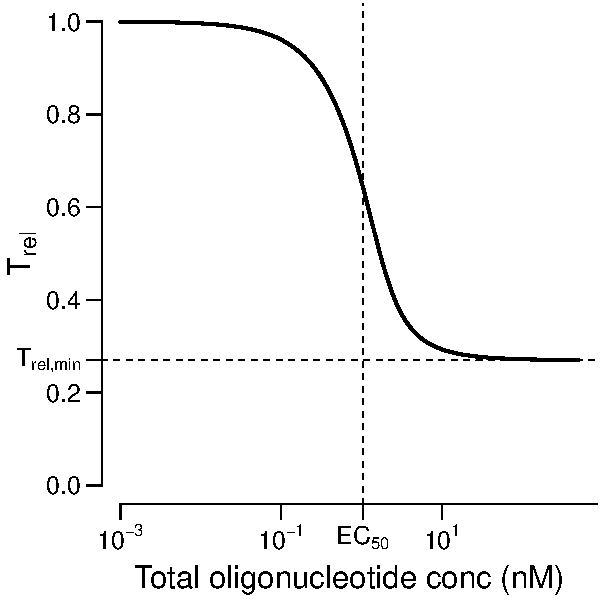
\includegraphics[width=0.5\textwidth]{Vignette2-Figc}
\end{Ncenter}
\caption{2c: The relative total target concentration ($\Trel$) is defined as the steady state level of total target in the presence of oligonucleotide divided by the target concentration in the absence of oligonucleotide. Dashed lines indicate 1-efficacy (horizontal) and $\EC$ (vertical).}
\end{figure}

%%%%%%%%%%%%%%%%%%%%%%%%%%%%%%%%%%%%%%%%%%%%%%%%%%%%%%%%%%%%%%%%%%%%%%%%%%
\subsection*{Figure 2d: An optimal affinity}
For a range of affinities \texttt{D1\_seq} the $\EC$-values are calculated by use of the R-function \texttt{EC50()} from the ASOmodels package:
\begin{Schunk}
\begin{Sinput}
> D1_seq <- 10^seq(-3,3.2,by=0.25)
> ECfit <- sapply(D1_seq,EC50)